\section{Multi-Agent Path Finding}
\label{sec:MAPF}
The \acrf{mapf} problem 


%
%
\subsection{Multi-Agent Pickup and Delivery}
The \acrf{mapd} is problem strictly relates to the \acrl{mapf} one. While \MAPF
aims at finding a feasible path for all the agents in the system from a
starting position to a desired destination, the \acrs{MAPD} problem introduces
the possibility for all the agent to have to meet an intermediate position.
Indeed, in industrial environment, robots usually need to complete a task by
starting from an initial position then moving to an intermediate one called
"pickup" location and finally to reach their delivery location. \newline
This introduces a remarkable difference from \MAPF, which can be seen as a
one-shot version of the problem~\cite{onlineMAPD}.\newline
Similarly to the for \MAPF, also the \acrs{MAPD} problem consists of $m$ agents
$\mathcal{A}=\{a_1,a_2,\hdots,a_m\}$ and an undirected connected graph 
$G=(V,E)$, where $V$ is the set of the vertices, i.e., the locations, and $E$
is the set of the edges, i.e., the connections between locations that the
agents can travel through. Let an agent $a_i$ start from a location $l_i(0)$,
then at each timestamp $t$, the agent either stays in the same position
$l_i(t+1)=l_i(t)$ or it moves to a neighboring node $(l_i(t), l_i(t+1))\in E$.
Moreover, as for the \MAPF problem, \textit{vertex} and \textit{swap} conflicts
should be avoided, that is two agents $a_i, a_j$ cannot be on the same node at 
the same time $l_i(t)\neq l_j(t)$ and they cannot move on the same edge at the
same time in opposite directions $l_i(t+1)\neq l_j(t) \wedge l_j(t+1)\neq
l_i(t)$, respectively. \newline
The part that mainly differs from the \MAPF problem is the fact that the agents
need to complete \textit{tasks}. A task $\tau_j$ can be defined as the tuple
$(s_j,g_j)$, where $s_j\in V$ is the pickup location and $g_j\in V$ is the 
destination to be reached. An agent is called \textit{free} at a certain moment
$t$ if it is not executing any task, otherwise it is called 
\textit{occupied}~\cite{onlineMAPD}. Notice that the agent is bound to a given
task from the moment it reaches the pickup location, i.e., if an agent $a_i$ is
associated with a task $\tau=(s, g)$, but has not reached $s$ yet, then another
agent $a_j$ may take over, e.g., when $a_j$ is closer to $s$ than $a_i$ is.
Consider a task set $\mathcal{T}$ in which the system inserts all the 
unexecuted tasks, then the goal of the problem is to execute all the tasks 
$\tau\in\mathcal{T}$.
\begin{figure}[tpb]
  \centering
  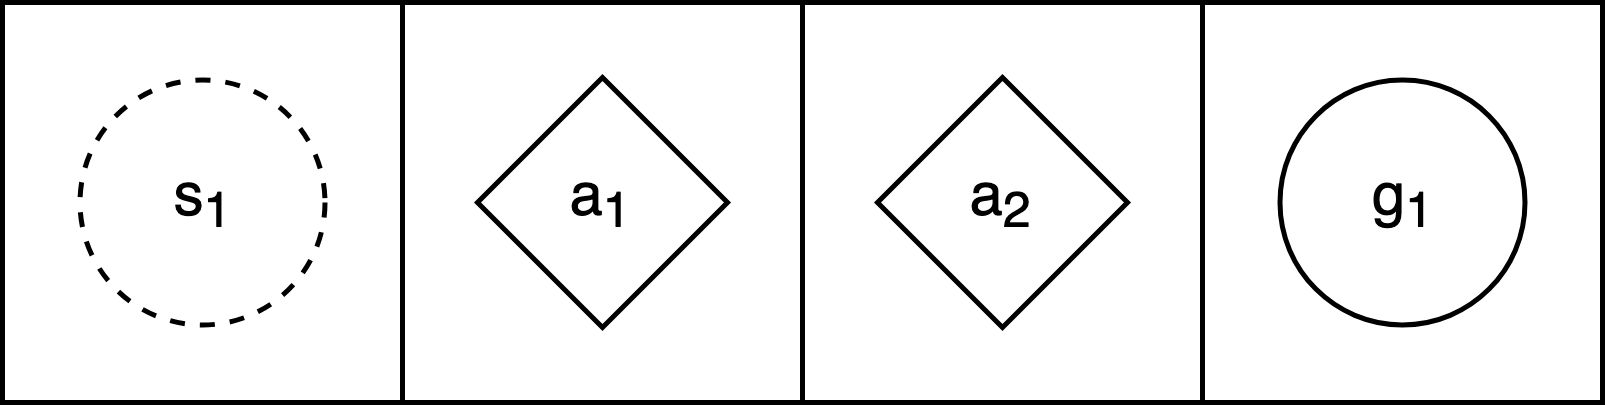
\includegraphics[width=0.4\textwidth]{onlineMAPD1}
  \caption{The figure shows a \acrs{MAPD} instance which is not solvable. The
  example shows an environment with two agents, $a_1, a_2$ and a task set
  $\mathcal{T}=\{\tau_1=(s_1,g_1)\}$. The instance is not solvable because 
  $a_2$ cannot move to $s_1$ without a vertex conflict and neither can $a_1$ 
  reach $g_1$ without a vertex conflict. }
  \label{fig:onlineMAPD1}
\end{figure}
\newline
The problem presented up until now it is as wide as possible. In this case,
there are instances that are not solvable, for example
Figure~\ref{fig:onlineMAPD1}. One possibility is to consider only well-formed,
or \textit{valid}, \acrs{MAPD} instances~\cite{wellFormedMAPD}. The idea is 
that agents can rest only on locations called \textit{non-task endpoints}, that 
is locations from where no other agent is blocked. \newline
One final distinction is done between \textit{offline} and \textit{online}
\acrs{MAPD} problems. The former assumes that all the tasks are known \textit{a 
priori} and no other task will be added to the task set during the execution of
the agents. Instead, the latter means that new tasks may continue to arrive and
that no information regarding the number of the tasks, nor their structure is
known \textit{a priori}. 
%
\subsubsection{Online MAPD Algorithms}
The state-of-the-art algorithms for solving the offline \acrs{MAPD} problem are
discussed in~\cite{onlineMAPD}, in which the authors presents two decoupled 
algorithms (\acrf{TP} and \acrf{TPTS}) and a centralized one called
\texttt{CENTRAL}. \newline
\acrs{TP} and \acrs{TPTS} use a token, i.e., a synchronized shared block of
memory, which contains the agents current paths, the task set and the agents
assignments. A central system is in charge to pass the token to the agents
which do the computations on their own. Indeed, the first step of the
algorithms consists in the system initializing the token with trivial paths in
which the agents stay on their initial locations. Then, whenever an agent has
reaches the end of the path as described in the token, it requests the token
from the system and chooses a new task to execute making sure that the pickup
and delivery locations of the new task do not produce a conflict with the other
agents paths. Two possibility may arise:
\begin{itemize}
  \item Such a task exists, then the agent chooses the task removing it from
    the task set and updates its path in the token trying to find a path that
    minimizes the cost while still avoiding collisions; or
  \item there is no such task, then it checks all the tasks in the task set to
    make sure that the its current position is not a delivery location. If it
    is not, then the token is updated with a stay path, otherwise an auxiliary
    function is called which will move the agent to a chosen endpoint without
    creating conflicts. 
\end{itemize}
\acrs{TPTS} adds to \acrs{TP} the possibility of swapping a task if the agent
assigned to it has not arrived to the pickup location yet. To do this, the task
set does not contain only unassigned tasks, but also unexecuted ones. If a task
$\tau$ is assigned to an agent $a_i$, but it is not yet been executed, then a
second agent $a_j$ can swap in and assign itself the task. For example, this
may be done when the latter agent can reach the pickup location in fewer steps 
than the former. When a swap happens, $a_j$ sends the token to $a_i$ which can
check if it can assign a new task to itself. 
